\documentclass[../main.tex]{subfiles}
\begin{document}

\section*{\centering 4. Animals and plants that live in aquatic habitat}
Mention the types of aquatic habitats and write about the plants and animals in aquatic habitats.\\[8pt]
\rotatebox{90}{\large Aquatic habitat}
    \fcolorbox{red}{white}{
		\begin{minipage}{\dimexpr\textwidth-15\fboxsep-4\fboxrule\relax}
			
        \begin{center}
        

\tikzset{every picture/.style={line width=0.75pt}} %set default line width to 0.75pt        

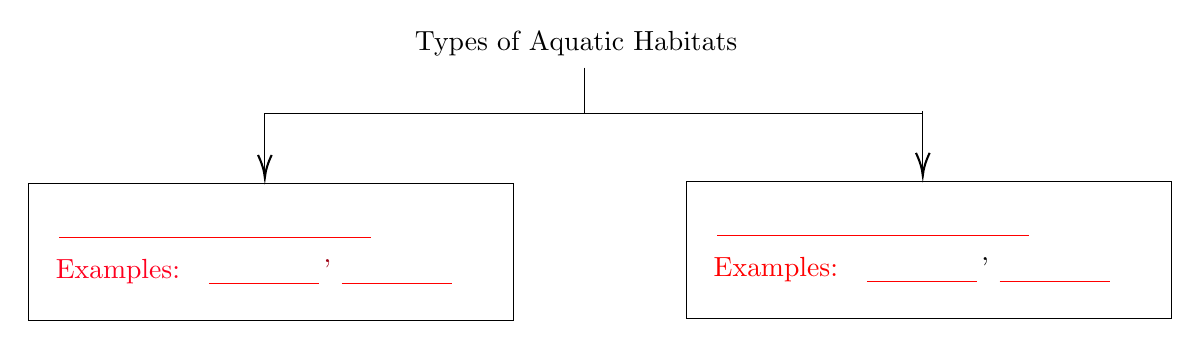
\begin{tikzpicture}[x=0.75pt,y=0.75pt,yscale=-1,xscale=1]
%uncomment if require: \path (0,300); %set diagram left start at 0, and has height of 300

%Straight Lines [id:da09508414902569307] 
\draw    (304,51) -- (304,73) ;
%Straight Lines [id:da6984252531733391] 
\draw    (150,73) -- (467,73) ;
%Straight Lines [id:da49090631642488136] 
\draw    (150,73) -- (150,102) ;
\draw [shift={(150,104)}, rotate = 270] [color={rgb, 255:red, 0; green, 0; blue, 0 }  ][line width=0.75]    (10.93,-3.29) .. controls (6.95,-1.4) and (3.31,-0.3) .. (0,0) .. controls (3.31,0.3) and (6.95,1.4) .. (10.93,3.29)   ;
%Shape: Rectangle [id:dp6260272318913588] 
\draw   (36,107) -- (270,107) -- (270,173) -- (36,173) -- cycle ;
%Straight Lines [id:da8585508401366753] 
\draw [color={rgb, 255:red, 255; green, 0; blue, 0 }  ,draw opacity=1 ]   (51,133) -- (201,133) ;
%Straight Lines [id:da14485769586688735] 
\draw [color={rgb, 255:red, 255; green, 0; blue, 0 }  ,draw opacity=1 ]   (123,155) -- (176,155) ;
%Straight Lines [id:da22746947464912148] 
\draw [color={rgb, 255:red, 255; green, 0; blue, 0 }  ,draw opacity=1 ]   (187,155) -- (240,155) ;
%Straight Lines [id:da22081169239397336] 
\draw    (467,72) -- (467,101) ;
\draw [shift={(467,103)}, rotate = 270] [color={rgb, 255:red, 0; green, 0; blue, 0 }  ][line width=0.75]    (10.93,-3.29) .. controls (6.95,-1.4) and (3.31,-0.3) .. (0,0) .. controls (3.31,0.3) and (6.95,1.4) .. (10.93,3.29)   ;
%Shape: Rectangle [id:dp030162788856562206] 
\draw   (353,106) -- (587,106) -- (587,172) -- (353,172) -- cycle ;
%Straight Lines [id:da24511754605870417] 
\draw [color={rgb, 255:red, 255; green, 0; blue, 0 }  ,draw opacity=1 ]   (368,132) -- (518,132) ;
%Straight Lines [id:da8247975010259052] 
\draw [color={rgb, 255:red, 255; green, 0; blue, 0 }  ,draw opacity=1 ]   (440,154) -- (493,154) ;
%Straight Lines [id:da33712526953657396] 
\draw [color={rgb, 255:red, 255; green, 0; blue, 0 }  ,draw opacity=1 ]   (504,154) -- (557,154) ;

% Text Node
\draw (221,32) node [anchor=north west][inner sep=0.75pt]   [align=left] {Types of Aquatic Habitats};
% Text Node
\draw (48,142) node [anchor=north west][inner sep=0.75pt]  [color={rgb, 255:red, 255; green, 0; blue, 31 }  ,opacity=1 ] [align=left] {Examples: };
% Text Node
\draw (177,142) node [anchor=north west][inner sep=0.75pt]  [color={rgb, 255:red, 158; green, 0; blue, 19 }  ,opacity=1 ] [align=left] {,};
% Text Node
\draw (365,141) node [anchor=north west][inner sep=0.75pt]  [color={rgb, 255:red, 255; green, 0; blue, 0 }  ,opacity=1 ] [align=left] {Examples: };
% Text Node
\draw (494,141) node [anchor=north west][inner sep=0.75pt]   [align=left] {,};
\end{tikzpicture}
        \end{center}
        \begin{minipage}[t]{0.48\textwidth}
        \textbf{Characteristics of aquatic animals:}
        \begin{enumerate}
          \item Shape - \underline{\hspace{3cm}}.
          \item Breathing organs of fishes in sea and river - \underline{\hspace{3cm}}.
          \item Breathing organs in whales - \underline{\hspace{3cm}}.
        \end{enumerate}
      \end{minipage}\hfill 
      \begin{minipage}[t]{0.48\textwidth}
        \textbf{Types of aquatic plants:}\\[6pt]
        \begin{tikzpicture}[inner sep=0pt]
            \node[anchor=north west] (img) at (0,0) {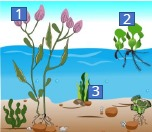
\includegraphics[width=4cm]{Task 5/images/plants.jpg}};
            \node[anchor=north west, text width=0.55\textwidth] at (4.2cm,0) {%
                \begin{enumerate}
                  \item \underline{\hspace{2cm}}
                  \item \underline{\hspace{2cm}}
                  \item \underline{\hspace{2cm}}
                \end{enumerate}
            };
        \end{tikzpicture}
    \end{minipage}
      \vspace{5pt} 
    \end{minipage}
	}
\end{document}